\documentclass[PMO,authoryear,toc]{lsstdoc}
% lsstdoc documentation: https://lsst-texmf.lsst.io/lsstdoc.html
%\input{meta}

% Package imports go here.

% Local commands go here.

%If you want glossaries
%\input{aglossary.tex}
%\makeglossaries

\title{CentOS System Disk Encryption}

% Optional subtitle
% \setDocSubtitle{A subtitle}

\author{%
Heinrich Reinking
}

\setDocRef{ITTN-048}
\setDocUpstreamLocation{\url{https://github.com/lsst-it/ittn-048}}

\date {\today}

% Optional: name of the document's curator
% \setDocCurator{The Curator of this Document}

\setDocAbstract{%
Disk encryption rises due to the need of protecting the information by converting it into unreadable code that cannot be deciphered easily. It uses hardware or software to encrypt bit by bit all data that goes on a disk. The Linux Unified Key Setup (LUKS) is a disk encryption software, that implements a platform-independent standard on-disk format for use in various tools.

The Policy-Based Decryption (PBD) is a collection of technologies that enable unlocking encrypted root and secondary volumes of hard drives on physical and virtual machines using different methods like a user password, a Trusted Platform Module (TPM) device, a PKCS11 device connected to a system, for example, a special network server. 
The PBD as technology allows combining different unlocking methods into a policy creating an ability to unlock the same volume in different ways. The current implementation of the PBD in Red Hat Enterprise Linux consists of the Clevis framework and plugins called pins. Each pin provides a separate unlocking capability. For now, the only two pins available are the ones that allow volumes to be unlocked with TPM or with a network server. 

The Network Bound Disk Encryption (NBDE) is a subcategory of the PBD technologies that allows binding the encrypted volumes to a special network server. The current implementation of the NBDE includes a Clevis pin for the Tang server and the Tang server itself.

Based on these tools, the Servers System Disk will be encrypted and when they boot, they will request decryption to a centralized server that withholds the Decryption key, avoiding the password prompt at boot.
}

% Change history defined here.
% Order: oldest first.
% Fields: VERSION, DATE, DESCRIPTION, OWNER NAME.
% See LPM-51 for version number policy.
\setDocChangeRecord{%
  \addtohist{1}{2021-05-09}{First Release}{Heinrich Reinking}
  \addtohist{2}{2021-06-01}{First Commit Concluded}{Heinrich Reinking}
  \addtohist{3}{2021-06-010}{Performance Test}{Heinrich Reinking}
}


\begin{document}

% Create the title page.
\maketitle
% Frequently for a technote we do not want a title page  uncomment this to remove the title page and changelog.
% use \mkshorttitle to remove the extra pages

% ADD CONTENT HERE
% You can also use the \input command to include several content files.
\lstset{ 
  backgroundcolor=\color{white},   % choose the background color; you must add \usepackage{color} or \usepackage{xcolor}; should come as last argument
  basicstyle=\footnotesize,        % the size of the fonts that are used for the code
  breakatwhitespace=false,         % sets if automatic breaks should only happen at whitespace
  breaklines=true,                 % sets automatic line breaking
  commentstyle=\color{green},      % comment style
  xleftmargin=2em,
  frame=single,
  framexleftmargin=1.5em,
  firstnumber=1,                   % start line enumeration with line 1000
  keepspaces=true,                 % keeps spaces in text, useful for keeping indentation of code (possibly needs columns=flexible)
  numbers=left,                    % where to put the line-numbers; possible values are (none, left, right)
  numbersep=4pt,                   % how far the line-numbers are from the code
  numberstyle=\tiny\color{gray},  % the style that is used for the line-numbers
  rulecolor=\color{black},         % if not set, the frame-color may be changed on line-breaks within not-black text (e.g. comments (green here))
  showspaces=false,                % show spaces everywhere adding particular underscores; it overrides 'showstringspaces'
  showstringspaces=false,          % underline spaces within strings only
  showtabs=false,                  % show tabs within strings adding particular underscores
  stepnumber=1,                    % the step between two line-numbers. If it's 1, each line will be numbered
  stringstyle=\color{red},         % string literal style
  tabsize=2,	                     % sets default tabsize to 2 spaces
}

\section{System Disk Encryption}
An encrypted system disk, prevents that the data contained in it can be clone or replicated without the passphrase or authentication server. For this design, the disks will be encrypted through kickstart passphrase and then removed once the remote Tang server are reached, which means, of non-authorized user gains physical access to the server:
\begin{itemize}
  \item Once the server boots, it will require root credentials.
  \item If halted and attempt to change the root password, the encryption passphrase prompt will be requested - which was deleted.
  \item If booted through a Live USB OS, the encrypted partitions remain unreadable.
  \item If the drive is taken, the disk would never gain access to its content.
\end{itemize}

\newpage
\subsection{LUKS - Linux Unified Key Setup}

According to a paper subscribed by Danut Anton and Emil Simion \footnote[1]{https://ieeexplore-ieee-org.usm.idm.oclc.org/stamp/stamp.jsp?tp=\&arnumber=8678978}, LUKS is one of the most common FDE solution for Linux based systems.
FDE works by encrypting every single bit on a storage device, so if the user doesn't have the password, data cannot be recovered. The most common problem for FDE solutions is password management, which at what concerns this implementation, will be handled by a two level key hierarchy. A strong master key is generated by an OS, which is used for encrypt/decrypt the hard drive. That key has to be split and encrypted with secret user key and stored on the device, at the beginning of the memory. The advantage of this approach is that you can have multiple systems with multiple keys, allowing you to have multiple decryption Servers.

\vskip 2cm
\begin{figure}
  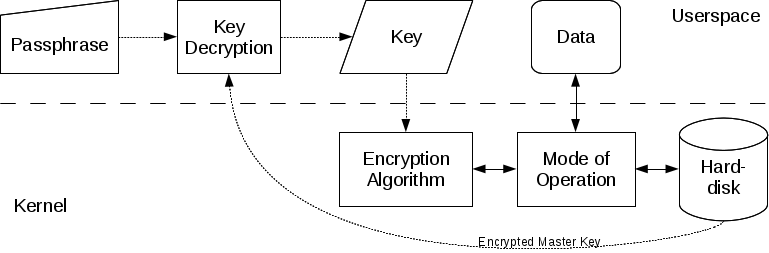
\includegraphics[width=14cm]{images/image2.png}
  \centering
  \caption{LUKS Operational Diagram}
\end{figure}

\newpage
\subsection{Clevis}

Clevis is a pluggable framework for automated decryption. It can be used to provide automate decryption of data or even automated unlocking of LUKS volumes \footnote[2]{https://github.com/latchset/clevis}.
To write: Clevis can subscribe up to 8 keys to 8 different servers/users and it can be restricted to how many of them are required as minimum; by default 1.


\subsection{Clevis Puppet Profile}
\begin{lstlisting}[language=Java]
#Clevis Profile
class profile::core::clevis() {
  $packages = [
    'clevis',
    'clevis-luks',
    'clevis-dracut'
  ]

  ##Add require packages
  package { $packages:
    ensure => 'present',
  }
  ->exec { '/sbin/dracut -f --regenerate-all':
    path   => ['/usr/bin', '/sbin'],
    onlyif => 'test ! -f /usr/lib/dracut/modules.d/60clevis/clevis-hook.sh'
  }
}
\end{lstlisting}

This profile install the clevis packages needed to encrypt and manage the LUKS encryption drives. This is not quite required, cause the clevis packages are being installed during provisioning, but, it grant some useful tools like 'cryptosetup' to check the subscribed Tang servers.

\newpage
\section{Tang Server - Decryption Server}

\subsection{Tang Service}

Tang \footnote[3]{https://github.com/latchset/tang} is a server for binding data to network presence. In simple terms: you have some data, but you only want it to be available when the system containing the data is on a certain, usually secure, network, This is where Tang comes in.
First the client gets a list of the Tang server's advertised asymmetric keys. This can happen online by a simple HTTP GET. 
Second, the client uses one of these public keys to generate a unique, cryptographically strong encryption key. The data is then encrypted using this key. Once the data us encrypted, the key is discarded. Some small metadata is produced as part of this operation which the client should store in a convenient location. This process of encrypting data is the provisioning step.
Third, when the client is ready to access its data, it simply loads the metadata produced in the provisioning step and performs an HTTP POST in order to recover the encryption key. This process of encrypting data is the provisioning step.

\vskip 2cm
\begin{figure}
  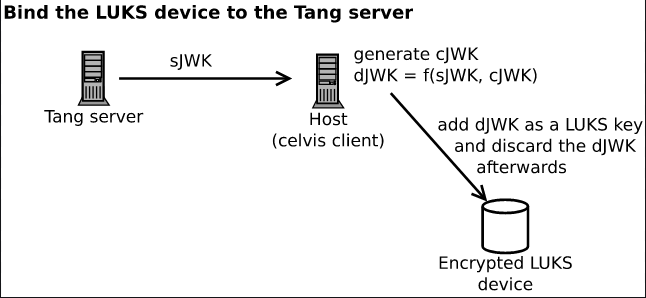
\includegraphics[width=14cm]{images/image3.png}
  \centering
  \caption{LUKS device interaction with Tang Server}
\end{figure}

\newpage
\subsection{Tang Puppet Profile and Role}

\begin{lstlisting}[language=Java]
#Tang Profile
class profile::core::tang() {
  #Variables
  $packages = ['tang']
  #Add require packages
  package { $packages:
    ensure => 'present',
  }
  #Ensure tang service is running
  service { 'tangd.socket':
    ensure  => 'running',
    require => Package[$packages],
  }
  #Create tangd.socket override directory
  file { 'tangd.socket.d':
    ensure => 'directory',
    path   => '/etc/systemd/system',
    mode   => '0755',
  }
  #Create override config file
  file { 'override.conf':
    ensure  => 'present',
    path    => '/etc/systemd/system/tangd.socket.d',
    mode    => '0644',
    require => File['tangd.socket.d'],
    content => @(OVERRIDE/L)
      [Socket]
      ListenStream=
      ListenStream=7500
      | OVERRIDE
  }
  ->exec { '/usr/bin/systemctl daemon-reload':
    refreshonly => true,
    notify      => Service['tangd.socket']
  }
}
\end{lstlisting}

Tang profile handles the installation of the tangd.socket service, and then modifies it so it listens on port 7500 for incomming connections from clevis-dracut.

\newpage
\section{Lab Testing - Proof of Concept}
\subsection{Kickstart Modifications - Use of Encryption in Provisioning Template}
Since the drive must me encrypted with LUKS early during the provisioning, new Kickstart Provisioning Template and Partition Tables had to be created at Foreman.

\vskip 0.5cm
\begin{lstlisting}[language=bash]
#Encrypted VDA - Partition Table

ignoredisk --only-use=${BOOT_DEV}
zerombr
clearpart --drives=${BOOT_DEV} --all --initlabel
part /boot     --size=1024 --asprimary --ondrive=${BOOT_DEV}
part /boot/efi --size=200  --asprimary --ondrive=${BOOT_DEV} --fstype=efi
part pv.boot   --size=1 --grow  --encrypted --passphrase=temppass --ondisk=${BOOT_DEV}
volgroup ${BOOT_VG} pv.boot
logvol /               --vgname=${BOOT_VG} --size=1 --grow --name=root
\end{lstlisting}

"Encrypted VDA" initialize the System disk with two regular partitions - /boot and /boot/efi - and then a PV, a VG and a LV, been the LV encrypted through LUKS with a temporary password
\begin{lstlisting}[language=bash]
##Kickstart - Encrypted Provisioning Template
#Packages Section
%packages
clevis-dracut
#Post Section
%post --log=/mnt/sysimage/root/install.post.log
curl -sfg http://tang01.cp.lsst.org/adv -o adv1.jws
clevis luks bind -f -k- -d /dev/vda3 \
tang '{"url":"http://tang01.cp.lsst.org","adv":"adv1.jws"}' <<< "temppass"
curl -sfg http://tang02.cp.lsst.org/adv -o adv2.jws
clevis luks bind -f -k- -d /dev/vda3 \
tang '{"url":"http://tang02.cp.lsst.org","adv":"adv2.jws"}' \ <<< "temppass"
cryptsetup luksRemoveKey /dev/vda3 <<< "temppass"
\end{lstlisting}

In the packages section, clevis-dracut is installed, to then be used at post to communicate with a Tang server(s), subscribe to them and remove the temporary password.

\newpage
\subsection{Test Environment}
\begin{itemize}
  \item Two Tang servers using the tang puppet profile.
  \item A client with the clevis puppet profile.
  \item The client VM (clevis01.cp.lsst.org) is provisioned through PXE with 'Encrypted VDA' Partitioning Table and 'Kickstart Encrypted Provisioning Template'.
  \item During partition creation, clevis01 root partition is encrypted through LUKS with the passphrase 'temppass'.
  \item Then at packages, clevis-dracut is installed to then communicate with the Tang servers at post section.
  \item At post, clevis01 subscribes to the Tang servers (tang01.cp.lsst.org and tang02.cp.lsst.org) and the temporary passphrase encryption key is removed as a decryption mechanism.
\end{itemize}

\begin{figure}
  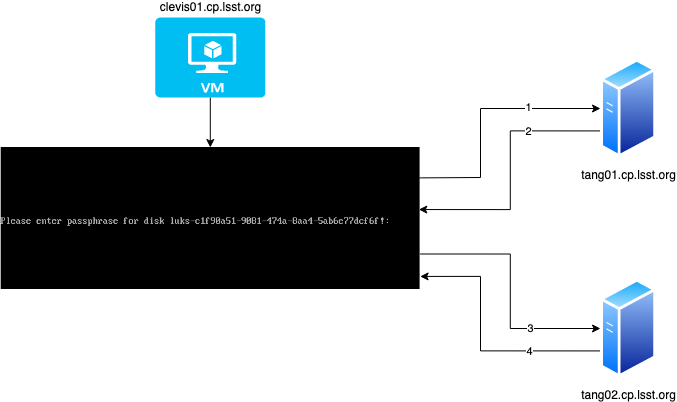
\includegraphics[width=10cm]{images/image4.png}
  \centering
  \caption{Booting procedure for an enrolled or newly enrolled client.}
\end{figure}

\begin{enumerate}
  \item During boot, the client machine attempts to reach first Tang server.
  \item If reached, the decryption server hands over the decryption key.
  \item If the first Tang server wasn't reachable, it attempts with the next one in the key slot.
  \item The second Tang server sends the decryption key.
\end{enumerate}

\newpage
\subsection{Lab Results}
\begin{itemize}
  \item The encrypted client clevis01 successfully decrypt during dracut by reaching tang01.
  \item The primary Tang server (tang01) was powered off and the client was able to decrypt through tang02.
  \item Both Tang servers were powered off and the server remains on hold requesting a passphrase (which doesn't exist) until at least one of the Tang servers is back online (Figure 3).
  \item For the scope of this PoC, the deletion and recreation of one or both Tang servers was not done, but presumably the client decryption would not happened and the content would be irrecoverable.
  \item One way of handling the loss of all Tang servers, is to add the keys to lsst-private repo, but key rotation is suggested by the documentation to increase safety.
\end{itemize}

\begin{figure}
  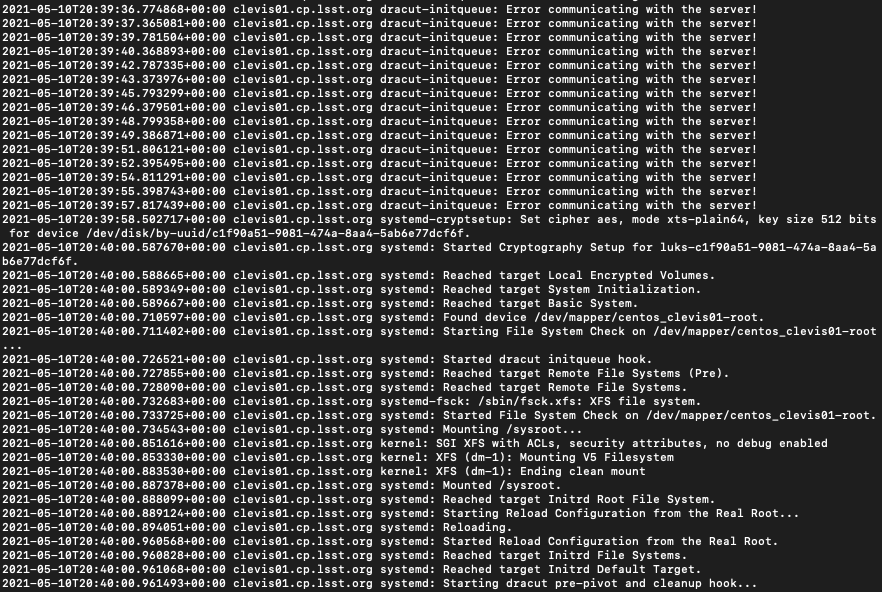
\includegraphics[width=16cm]{images/image1.png}
  \centering
  \caption{Access to LUKS encrypted drive while Tang server is rebooting}
\end{figure}

\newpage
\subsection{Conclusions - Pros and Cons}
\begin{itemize}
  \item The system disk MUST be encrypted during the provisioning, meaning that systems that have already been provisioned cannot be encrypted without risking data loss.
  \item Disk decryption successfully proved with the usage of Clevis - on the client side - and Tang - on the server side -. 
  \item During boot, it starts the network interface and contacts the Tang server for automated decryption.
  \item Since this occurs during provisioning, puppet cannot handle the root partition encryption, only if it was a non-root partition.
\end{itemize}


\newpage
\appendix
% Include all the relevant bib files.
% https://lsst-texmf.lsst.io/lsstdoc.html#bibliographies
%\section{References} \label{sec:bib}
\renewcommand{\refname}{} % Suppress default Bibliography section
\bibliography{local,lsst,lsst-dm,refs_ads,refs,books}

% Make sure lsst-texmf/bin/generateAcronyms.py is in your path
\newpage
\section{Acronyms} \label{sec:acronyms}
\addtocounter{table}{-1}
\begin{longtable}{p{0.145\textwidth}p{0.8\textwidth}}\hline
\textbf{Acronym} & \textbf{Description}  \\\hline

FDE & Full Disk Encryption \\\hline
GPFS & General Parallel File System \\\hline
HDD & Hard Drive Disk \\\hline
LUKS & Linux Unified Key Setup \\\hline
LV & Logical Volume \\\hline
NBDE & Network Bound Disk Encryption \\\hline
OS & Operating System \\\hline
PBD & Policy-Based Decryption \\\hline
PV & Physical Volume \\\hline
PoC & Proof of Concept \\\hline
SSD & Solid State Drive \\\hline
TPM & Trusted Platform Module \\\hline
VDA & Virtual Drive A \\\hline
VG & Volume Group \\\hline
\end{longtable}

% If you want glossary uncomment below -- comment out the two lines above
%\printglossaries

\end{document}